%\newpage
\subsection{System Design}
\subsubsection{System Architecture}
\begin{figure}[H]\centering
  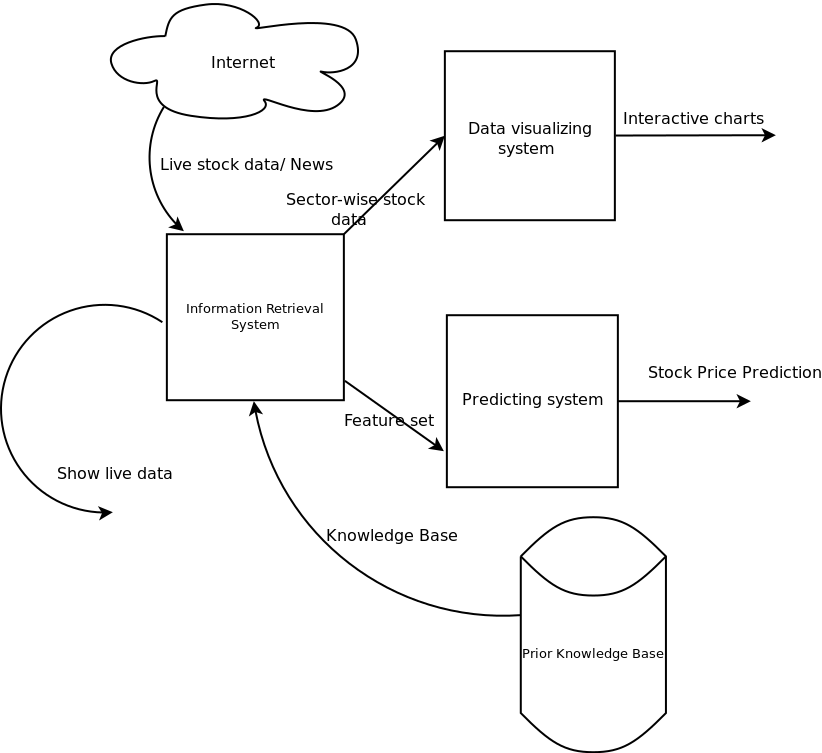
\includegraphics[width=5in]{fig/System}
  \caption{Overall system architecture}
  \label{fig:System}
\end{figure}

\subsubsection{UML Diagrams}
\begin{figure}[H]\centering
  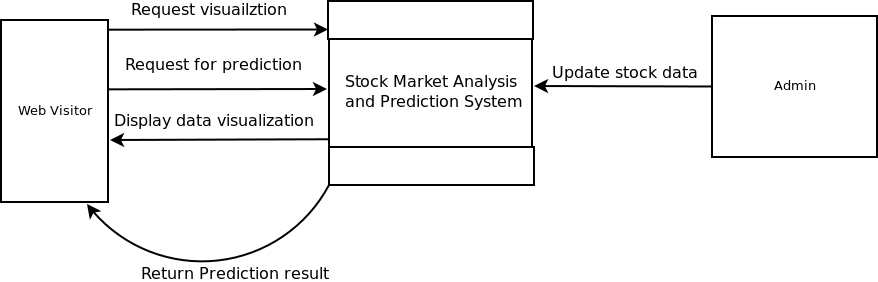
\includegraphics[width=6in]{fig/Dfd1}
  \caption{Level-1 dataflow diagram (DFD)}
  \label{fig:Dfd1}
\end{figure}

~

\begin{figure}[H]\centering
  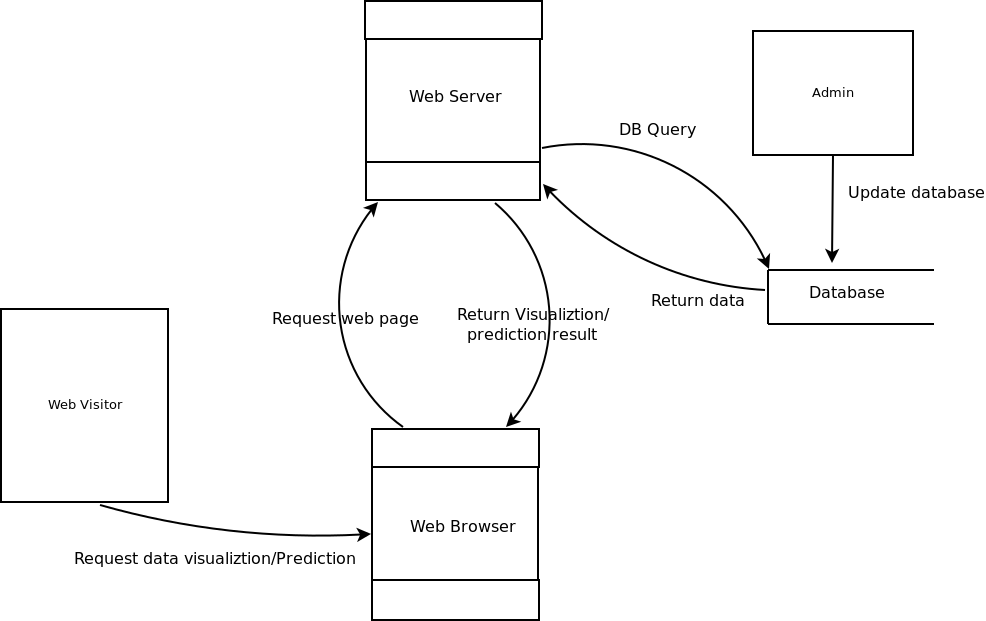
\includegraphics[width=6in]{fig/DFD2}
  \caption{Level-2 dataflow diagram (DFD)}
  \label{fig:DFD2}
\end{figure}


\begin{figure}[H]\centering
  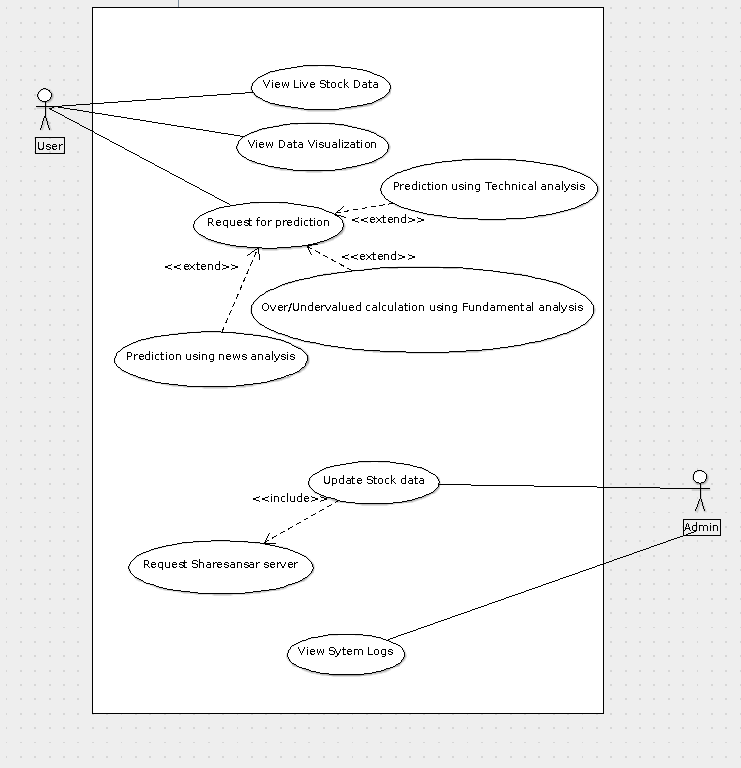
\includegraphics[width=6.5in]{fig/usecase2}
  \caption{Use case diagram}
  \label{fig:usecase2}
\end{figure}

\begin{figure}[H]\centering
  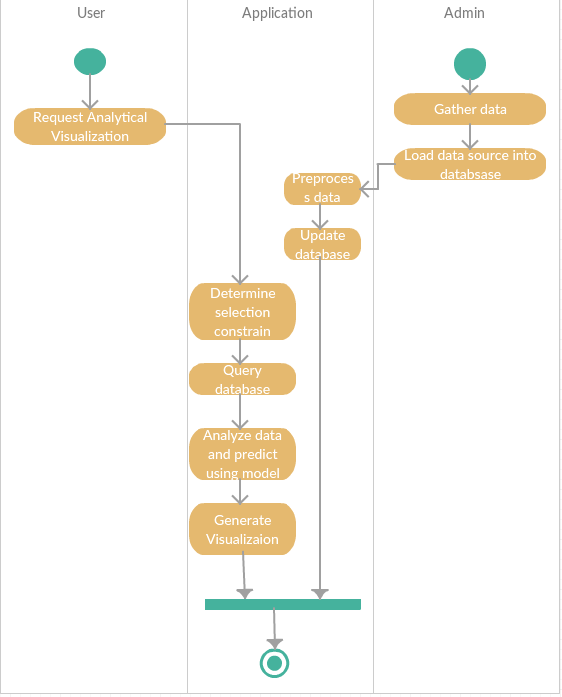
\includegraphics[width=6.5in]{fig/activity}
  \caption{Activity diagram}
  \label{fig:activity}
\end{figure}

\begin{figure}[H]\centering
  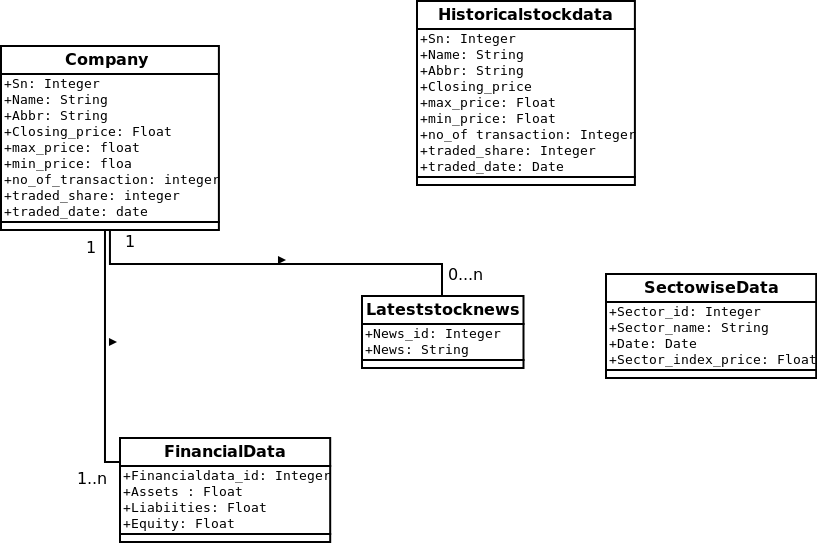
\includegraphics[width=6in]{fig/classdiagram}
  \caption{Class diagram}
  \label{fig:classdiagram}
\end{figure}

~

\begin{figure}[H]\centering
  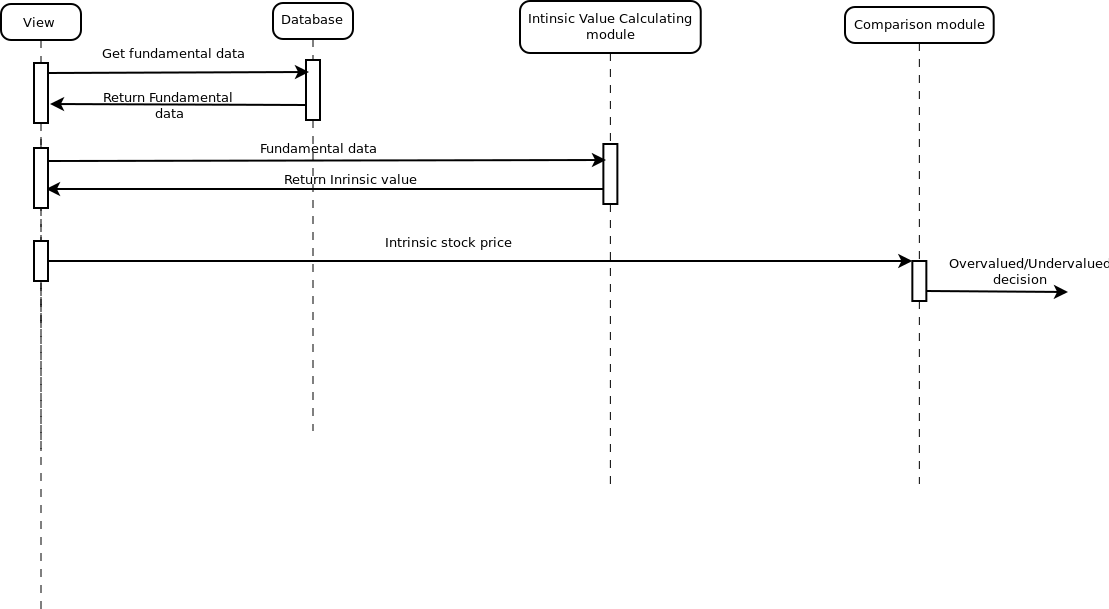
\includegraphics[width=\textwidth]{fig/fundamental}
  \caption{Sequence diagram for Fundamental Analysis}
  \label{fig:Fundamental}
\end{figure}

\begin{figure}[h!]
  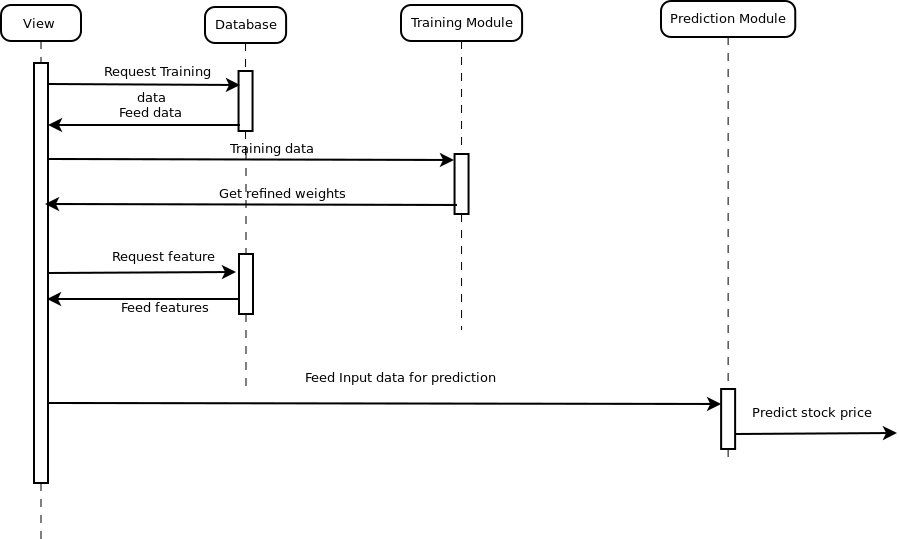
\includegraphics[width=\textwidth]{fig/StockPredictionusingNN}
  \caption{Sequence diagram For technical analysis using NN }
  \label{fig:StockPredictionusingNN}
\end{figure}

~


\begin{figure}[H]\centering
  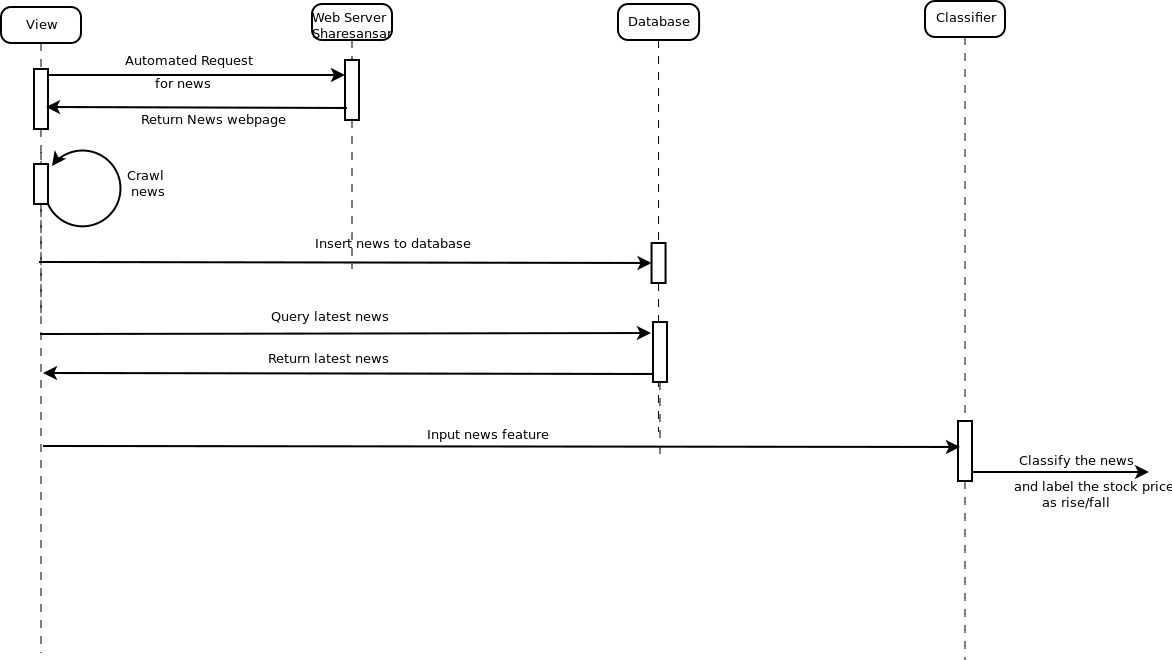
\includegraphics[width=6in]{fig/newsanalysis}
  \caption{Sequence diagram for New Analysis}
  \label{fig:newsanalysis}
\end{figure}

\begin{figure}[H]\centering
  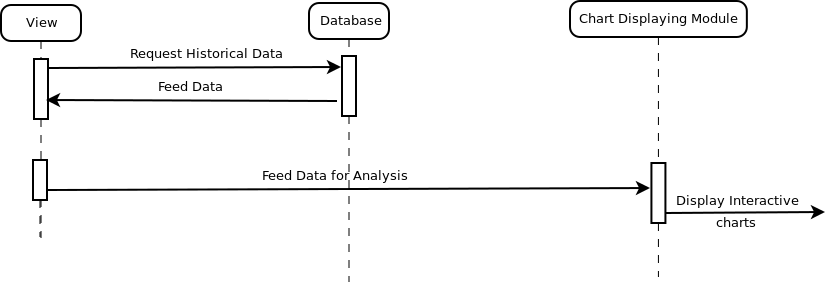
\includegraphics[width=6in]{fig/Charting}
  \caption{Sequence diagram for Data Visualization}
  \label{fig:Charting}
\end{figure}



